\section{User manual}

\subsection{Functional requirements}
\begin{itemize}
\item Requires the user to have an Android device with Android OS v2.2 or newer.
\item Requires internet connection to be able to play online.
\end{itemize}

\subsection{Running the application}
The project files are supplied with the delivery. The project can be run in an emulator or on an Android device. In both scenarios it is recommended to open the project in Eclipse. It can also be installed directly on an Android device with the supplied *.apk file.

\subsubsection{Opening project in Eclipse}
Opening the project in Eclipse is done as follows:
\begin{enumerate}
\item Choose \emph{File}
\item Choose \emph{Open project}
\item Choose \emph{Existing source code}
\item Navigate to the download path, and open the project
\end{enumerate}
%File -> Open project -> Existing source code -> path to downloaded project.

\subsubsection{Running in emulator}
To run the project in an emulator, the user needs to install an AVD, and then choose to run the project with this AVD.

\subsubsection{Running on device}
The user needs to connect the Android device to the computer, and run the project with the device set as target.

\subsubsection{Installing APK-file}
The user needs to connect the Android device to the computer, and transfer the APK-file to the SD card. The settings on the device must be set to accept installing applications from unknown sources. The next step is to open the file browser on the device, and click the application file on the SD card. It will then prompt the user to install the application.

\subsection{Game rules}
The game is implemented with the same set of rules as the classic board game \emph{Nine Men's Morris} \cite{morris}. The goal of the game is to either block any opponent moves, or to reduce your opponent's piece number to less than three. If you get three pieces in a row, you enter a morris state, and are allowed to remove one of your opponent's pieces. Pieces that are in a morris state, i.e. forms three in a row either horizontally or vertically, are not removable.

\subsection{Creating Skiller account}
When running the application, the user is prompted to create a Skiller user account. The registration only requires a username and a password. If the user already has an account, he can log in with the existing user information. The account automatically gets 50 coins.

\subsection{How to play}
\label{section:playing}

\subsubsection{Choosing game mode}
A user can choose between online mode or hotseat mode. Clicking "Crate Game" or "Join Game" will start a game in online mode. Clicking "Hotseat" will start a game in hotseat mode.
\label{section:game_mode}
\begin{figure}[H]
	\centering
	\mbox{
	\subfigure[Available game modes]{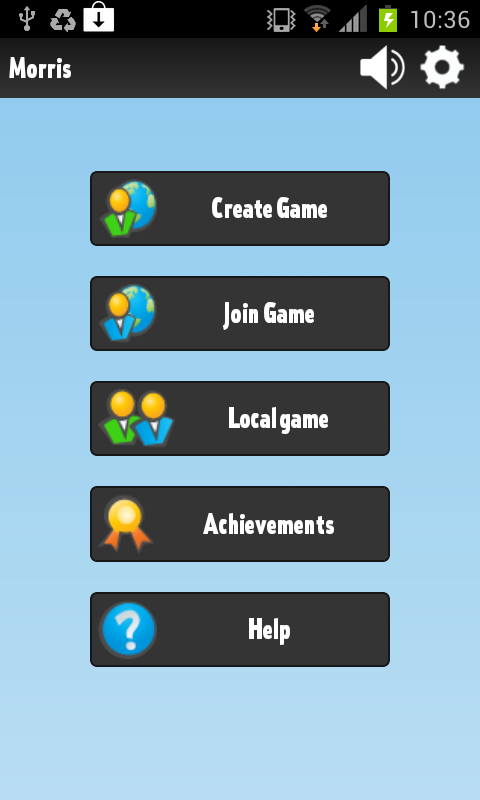
\includegraphics[width=0.3\textwidth]{Images/menuPage.png}}
	\subfigure[Achievements]{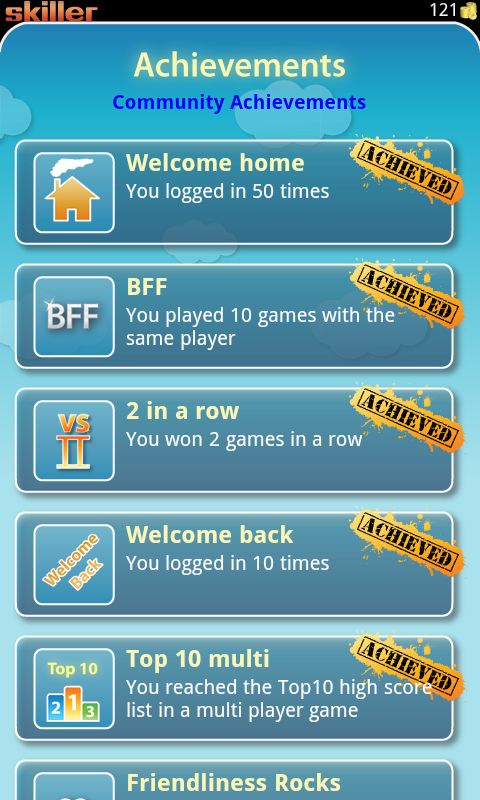
\includegraphics[width=0.3\textwidth]{Images/achievements.png}}
	\subfigure[Help explaining the games rules]{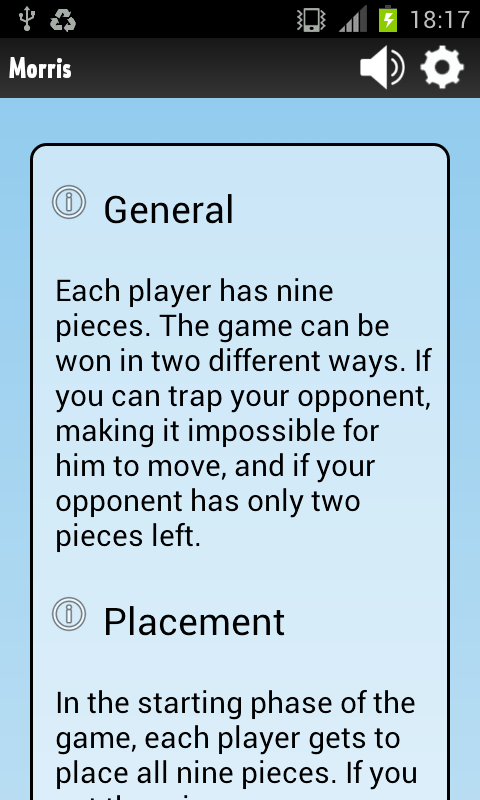
\includegraphics[width=0.3\textwidth]{Images/help.png}}
	}	
\end{figure}

\subsubsection{Placing, selecting, moving, and removing pieces}
When it is your turn to move, either the board or your pieces will be highlighted. In addition, the name of the current player will be blinking as the game progresses. \\
\begin{figure}[H]
	\centering
	\mbox{\subfigure[Green indicator shows where you can place a piece]{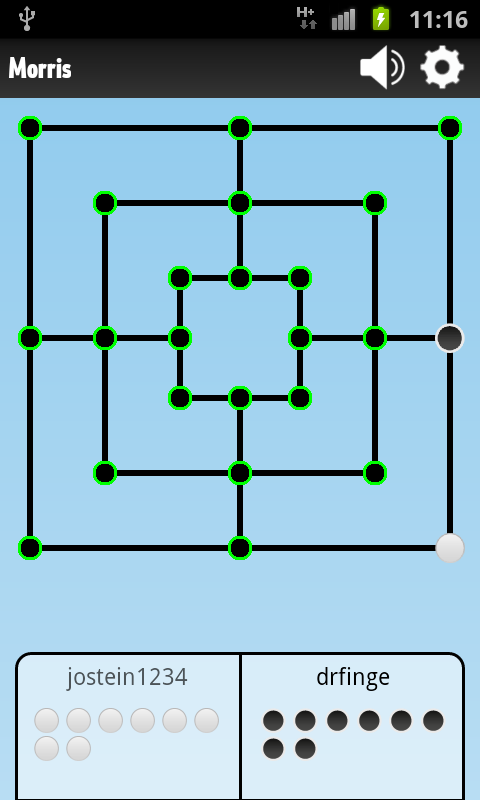
\includegraphics[width=2.1in]{Images/placementState.png}} \qquad
	\subfigure[Highlights selectable pieces]{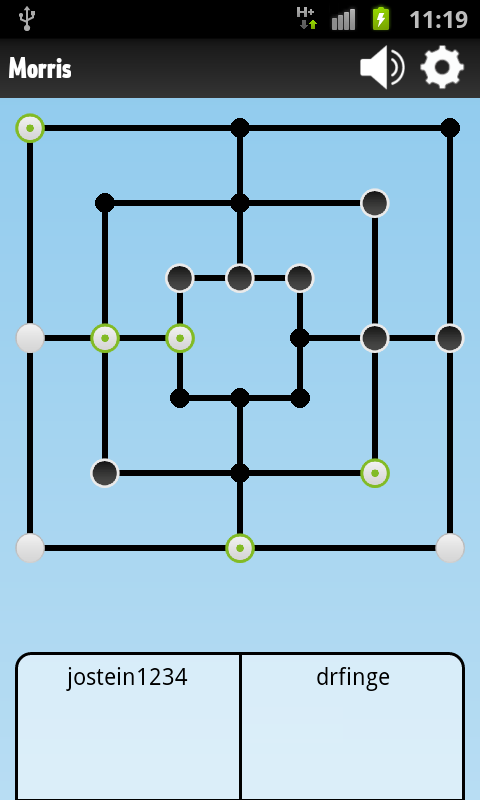
\includegraphics[width=2.1in]{Images/selectState.png}}}
	\mbox{\subfigure[Highlight selected piece, green indicator on possible moves]{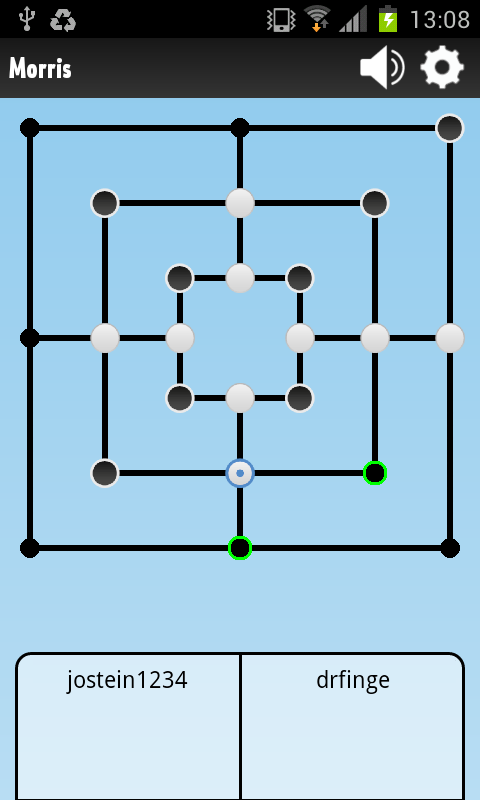
\includegraphics[width=2.1in]{Images/selectedPiece.png}} \qquad
	\subfigure[Highlights removable pieces with a red cross]{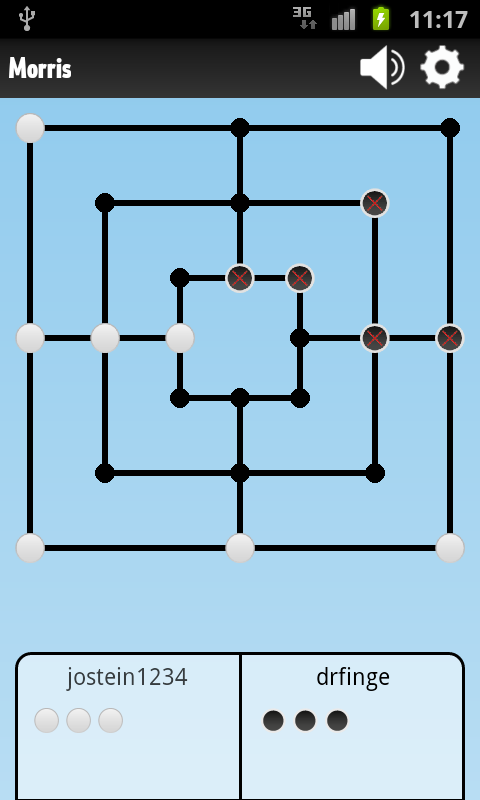
\includegraphics[width=2.1in]{Images/removalState.png}}}
\end{figure}

\subsubsection{Hotseat mode}

If you start a local game as described in section \ref{section:game_mode}, you can control both players from the same device.

\subsubsection{Online mode}

If you start an online game as described in section \ref{section:game_mode}, you are taken to the board screen, and need to wait for another player to join your game. The guest, i.e. the one who joins the game, will get the initial move. Your own pieces will always be white.






